\documentclass[11pt]{article}
\usepackage[super,square,comma]{natbib}
\usepackage[letterpaper, margin=1.25in]{geometry}
\usepackage{tikz}
\usepackage{lipsum}
\usepackage{setspace}
\usepackage{enumerate}
\usepackage[inline, shortlabels]{enumitem}
\usepackage{amsmath}
\newtheorem{problem}{Problem}
\numberwithin{equation}{section}

\usepackage{animate}
\usepackage{siunitx}
\usepackage{csquotes}
\usepackage{graphicx}
\usepackage{authblk}
\usepackage[labelfont=bf]{caption}
\usepackage{subcaption}

\usepackage{fancyhdr}
\pagestyle{fancy}
\lhead{Team 93463}
\chead{\textsc{Multi-hop, HF Radio Propagation Near Japan}}
\rhead{Page \thepage\ of \pageref{LastPage}}
\setlength{\headheight}{14pt}

\usepackage{lastpage}

\renewcommand{\thefootnote}{\arabic{footnote}}
\newcommand{\cn}{$^{\text{[citation needed]}}$} %citation needed

% %%% Title Page Author Stuff %%%
% \renewcommand*{\Authsep}{, }
% \renewcommand*{\Authand}{, }
% \renewcommand*{\Authands}{, }
% \renewcommand*{\Affilfont}{\normalsize\normalfont}
% % \renewcommand*{\Authfont}{\bfseries}    % make author names boldface    
% \setlength{\affilsep}{1em}   % set the space between author and affiliation

% \newsavebox\affbox

% \author[1]{Colin M. Adams}
% \author[1]{Rachel L. Barcklay}
% \author[1,2]{Carla J. Becker}
% \affil[1]{%
%   \savebox\affbox{\Affilfont Department of Physics, Harvey Mudd College}%
%   \parbox[t]{\wd\affbox}{\protect\centering Department of Physics, Harvey Mudd College}} 
% \affil[2]{Department of Chemistry, Harvey Mudd College \par Claremont, CA 91711}



%%%%%%%%%%%%%%%%%%%%%%%
\renewcommand{\baselinestretch}{2}
\newcommand{\shrug}[1][]{%
\begin{tikzpicture}[baseline,x=0.8\ht\strutbox,y=0.8\ht\strutbox,line width=0.125ex,#1]
\def\arm{(-2.5,0.95) to (-2,0.95) (-1.9,1) to (-1.5,0) (-1.35,0) to (-0.8,0)};
\draw \arm;
\draw[xscale=-1] \arm;
\def\headpart{(0.6,0) arc[start angle=-40, end angle=40,x radius=0.6,y radius=0.8]};
\draw \headpart;
\draw[xscale=-1] \headpart;
\def\eye{(-0.075,0.15) .. controls (0.02,0) .. (0.075,-0.15)};
\draw[shift={(-0.3,0.8)}] \eye;
\draw[shift={(0,0.85)}] \eye;
% draw mouth
\draw (-0.1,0.2) to [out=15,in=-100] (0.4,0.95); 
\end{tikzpicture}}


\title{
    \textsc{{Multi-hop, High-Frequency Radio Propagation Near Japan}}
    }

\author{\Large Team 93463}
\date{\today}
        

\begin{document}
%%%%%%%%%%%%%%%%%%%%%%%%%%%%%%%%%%%%%%%%%%%%%%%%%%%%%%%%%%%%%%%%%%%%%%
% Title Page
%%%%%%%%%%%%%%%%%%%%%%%%%%%%%%%%%%%%%%%%%%%%%%%%%%%%%%%%%%%%%%%%%%%%%%
    \singlespacing %sets spacing of abstract to single
    \clearpage 
    \maketitle
    \thispagestyle{empty} %gets rid of page number at bottom 

    To whom it may concern, \\
    When reading our solution, we hope that you are can read our document in Adobe Acrobat Reader as we have \texttt{.gif} files that can only play with that PDF reader. Please visit \texttt{https://get.adobe.com/reader/} to download it if need be. It is worth it. We promise.
    \begin{center}
        \rule{11cm}{0.4pt}  
    \end{center}

\begin{abstract}
    Hi team, here is what we \emph{need} to have in our report (according to the MCM overlords):
\begin{itemize}
    \item Restatement and clarification of the problem
    \item Explain assumptions and rationale/justification
    \item Include your model design and justification
    \item Describe model testing and sensitivity analysis
    \item Discuss the strengths and weaknesses
\end{itemize}

They also claim to judge the quality of our writing. So remember our good friend Williams. \shrug\cite{townsend2000modern}
\end{abstract}
\newpage

%%%%%%%%%%%%%%%%%%%%%%%%%%%%%%%%%%%%%%%%%%%%%%%%%%%%%%%%%%%%%%%%%%%%%
%% Body
%%%%%%%%%%%%%%%%%%%%%%%%%%%%%%%%%%%%%%%%%%%%%%%%%%%%%%%%%%%%%%%%%%%%%
\setcounter{page}{1} %set new page number to 1

\section{Motivation} % (fold)
\label{sec:motivation}

Quickly after its invention in the late 19th century, radio was adopted worldwide as the main form of communication for long distances near instantaneously.\cite{hilmes2002radio} When utilized correctly, the radio has accomplished remarkable things. Radios have inspired generations of scientists and tinkerers; they have allowed world-leaders to communicate with their people, soldiers to their brothers-in-arms,\footnote{Yes, we know. This terminology is a little dated.} they have allowed music to spread across cultures, and they have allowed Alex Jones spout gibberish to conspiracy theorists across the United States.\footnote{Enjoy. \texttt{https://youtu.be/aCiVsJ3b160}} 

However, the often the catastrophic failures of radio have been a result of not understanding the science behind them. For example, a poor understanding of the Titanic's radio contributed to the deaths of 1,514 passengers and crew from April 14--15, 1912.\cite{noauthor_radio_2011} While much---if not most---of the engineering difficulties of radio have been overcome, some of the fundamental science behind it has not, e.g. ground-wave propagation.\cite{budden1961radio} To avoid other horrendous accidents at sea, such as the Titanic, it's important to have an accurate model of how radio-waves propagate through the atmosphere to determine the maximum distance a signal can travel at sea.

Our task, if we choose to accept it,\footnote{Cue the Mission Impossible theme song: Dun Dun Dun da dada Dun dun dun da dada dun dun dun da dada, de da doo de da doo de da doo do dut.} is to solve the following three problems:
\begin{problem}
 The first problem we are trying to solve is to determine how many times a HF radio-wave can be reflected off of the ocean. The first reflection of the signal is off of a turbulent ocean. We must characterize how the signal strength changes after this first reflection. After the first reflection, we are looking to characterize how the signal changes as it reflects off of calm oceans before falling below a signal to noise ratio (SNR) of 10\,\si{\dB}.
 \label{pr:turb_ocean}
\end{problem}

\begin{problem}
    This is the same problem as Problem \ref{pr:turb_ocean}, but instead of the ocean, we have rugged and smooth terrain.
    \label{pr:mount}
\end{problem}

\begin{problem}
    Lastly, we would like to see how a boat traveling across the ocean using HF radio-waves to communicate and how our model changes to accommodate a receiver in motion on a turbulent ocean.
    \label{pr:boat}
\end{problem}
% section motivation (end)

\section{Introduction} 
\label{sec: intro} 

 \begin{figure}[ht]
 \begin{center}
     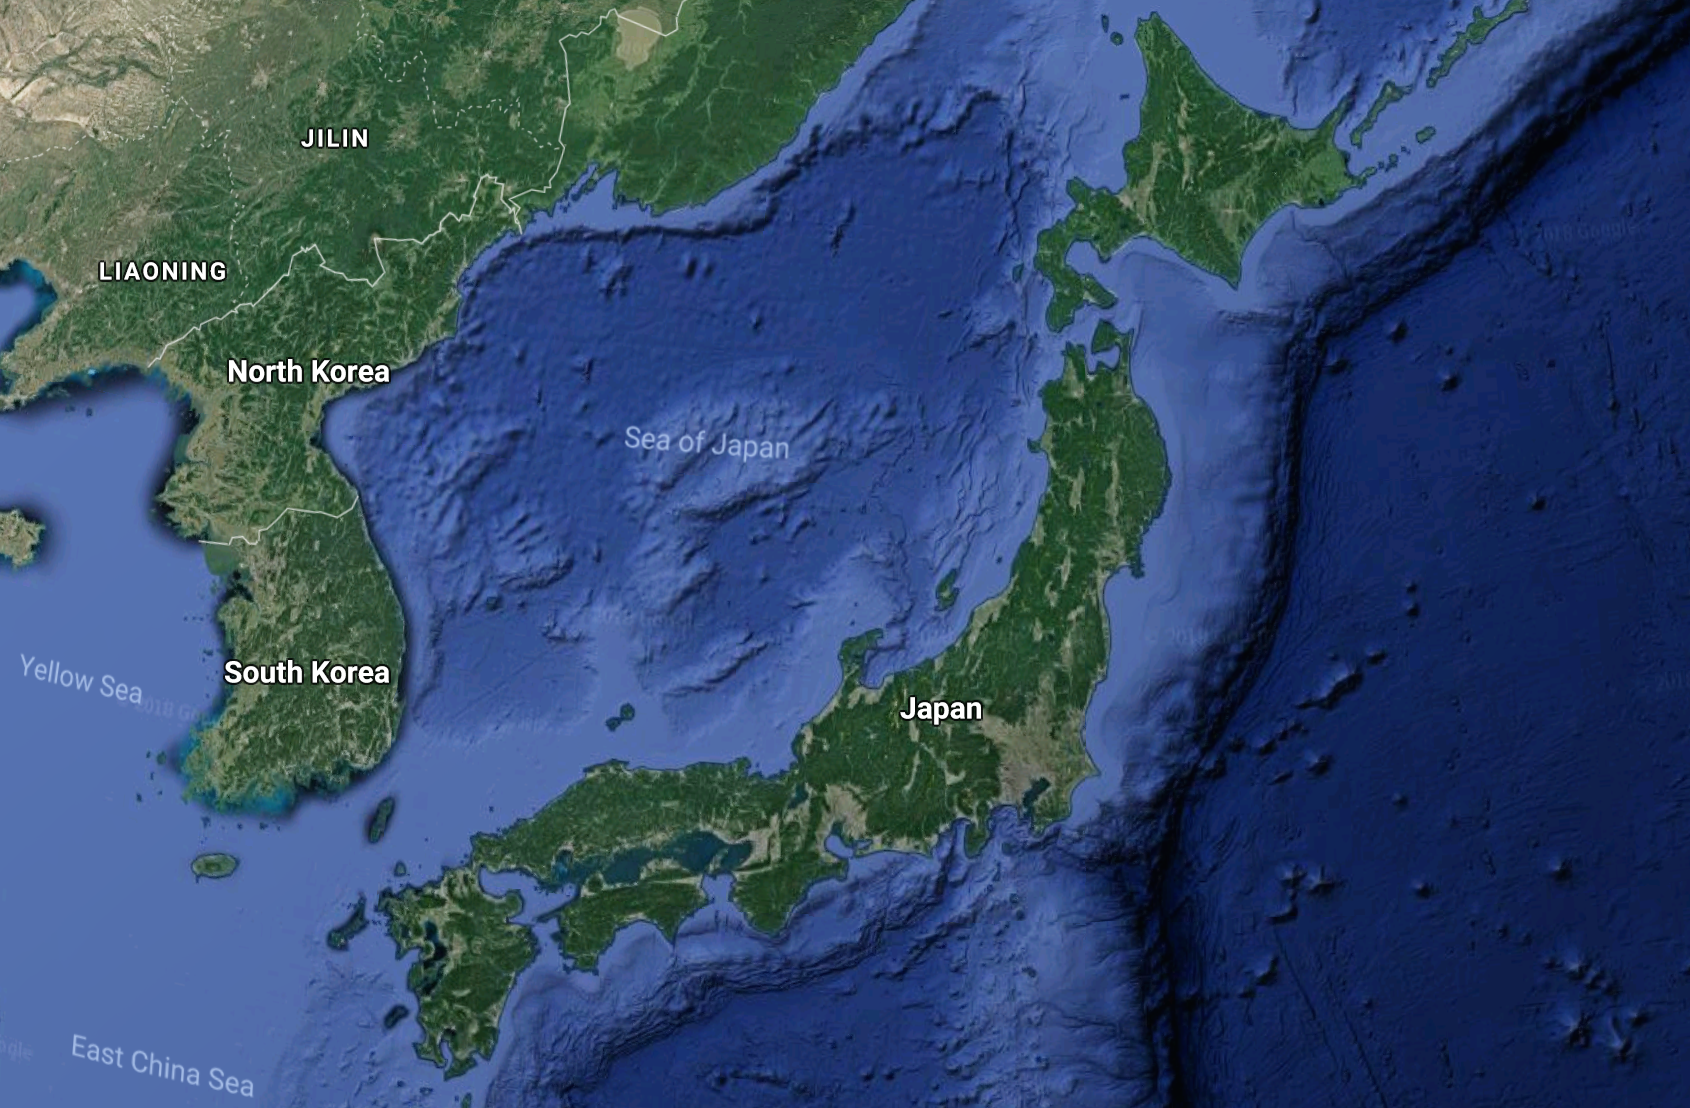
\includegraphics[width = 4.55in]{figs/japan.png}
 \end{center}
 \caption{The region we are studying of choice. Japan was chosen due to it being an island surrounded by ocean water and it is a very mountainous and rugged country. Image taken from Google Maps.}
 \label{fig:jap} 
\end{figure} 

High frequency radio-waves (defined to be between 3--30\,\si{\mega\hertz}) can travel through the atmosphere---by one mechanism---by multiple reflections off of the Earth's ionosphere and the its surface. For frequencies below the maximum usable frequency (MUF), they will skip from the surface of the earth to the ionosphere and back again indefinitely until the signal dies down and becomes unusable. If the frequencies are larger than the MUF, then they pass through the ionosphere and are lost to space forever. The MUF varies with the season, time of day, and solar conditions.\cite{mcm_statement} In our model, we will neglect solar conditions for simplicity.


Empirically, radio-waves reflect off of the ocean differently depending on whether the ocean is turbulent or calm, impacting the distance the signal can faithfully.\cite{mcm_statement} Not surprisingly, radio-waves will reflect off rugged terrain differently than smooth, making it important to model how these radio-waves travel over mountains as well.

With this in mind, we decided to focus on a region of with a radius of roughly 550\,\si{\km} from Tokyo, Japan (Fig.\ref{fig:jap}). We chose this location because there is a large quantity of reliable data taken in Japan, it is an island country, and is ``mostly rugged and mountainous.''\cite{factbook2010world} In essence, it is an ideal location to accurately study high-frequency (HF) radio-waves and their interactions with ionosphere and ocean.


\section{Model} % (fold)
\label{sec:model}

To have an accurate model, there are three main components of this model that need to be described. Primarily, we need to be able to describe HF radio-waves and how they change with reflections and gather inherent noise gathered as it travels through a medium. Because our signal reflects off of two different interfaces as it travels---the ocean and the ionosphere---it is important to model each with accurate physical properties. We would like to see how they change with time of day and time of year. 
\subsection{Radio-waves} % (fold)
\label{sub:radiowaves}

 \begin{figure}
     \begin{center}
        \animategraphics[width=4.25in]{12}{gif/frame-}{0}{99}
     \end{center}
     \caption{A test \texttt{.gif} file. Click image to see animation. \\\\You need to use Adobe Acrobat Reader to view. If you do not have it, please visit \texttt{https://get.adobe.com/reader/} to download it. It is worth it.}
 \end{figure}

\subsubsection{Noise} % (fold)
\label{ssub:noise}

As radio-waves propagate over a certain distance, we expect them to pick up some noise as they go, degrading the integrity of the information they are trying to transmit. If they didn't, you could presumably use a \$5 hand-held radio to communicate with police officers in Australia.\footnote{It doesn't. One of the authors tried as a child.} A reasonable question becomes, how should we try and model this.

The Central Limit Theorem states that when using independent, random variables\footnote{We are assuming this in our model.} are added together, their properly normalized sums tend toward a normal distribution.\cite{central} So as the radio-wave travels, we add this Gaussian noise to the signal to degrade it as its path length increases. It turns out that this is used quite often in Information Theory, and is called Additive White Gaussian Noise (AWGN).\cite{shannon1984communication,kailath1968innovations}

% subsubsection noise (end)
% subsection radiowaves (end)

\subsection{The Ionosphere} % (fold)
\label{sub:the_ionosphere}

The ionosphere consists of roughly three layers that lie between 75--1000\,km above the Earth's surface:
\begin{enumerate*}[(1)]
    \item the F-region,
    \item the E-region, and
    \item the D-region
\end{enumerate*}; each of these regions has charge-density dependent on the time of year, the number of sunspots present, the time of day, and the movement of the charged particles\footnote{The study of which has the impressive sounding name of magnetohydrodynamics.}(Figure \ref{fig:struct_ion}). X-rays, ultraviolet light, ejected plasma, and other high energy particles that are released by the sun interact with the atoms in the atmosphere and strip them of electrons.\cite{noauthor_tracking_nodate} The ionosphere interacts heavily with radio waves, mainly through the interaction of these free electrons.\cite{budden1961radio}

Early experiments demonstrated that the electrons in the ionosphere are arranged in approximately horizontal layers, meaning that the number density is a function of height above the Earth's surface. Presumably, these cations are  atoms or molecules stripped of an electron. Because the ratio between the mass of a proton (the smallest positive charge we could have in the atmosphere) and an electron is on the order of $2\times10^3$, we would expect there must be approximately $5 \times10^{-4}$ more cations than electrons.\footnote{This is because the electric field of the propagating radio-waves will have $5 \times10^{-4}$ of the effect on a proton than an electron because its acceleration $\mathbf{a} \propto 1/m$.} If this were the case, the ionosphere would be unstable, due to the large repulsive forces of this unbalanced positive charge. However, due to the ionosphere's empirically determined and stable layers, the ionosphere must be nearly electrically neutral, i.e. there must be an equal number of positive and negative charges per unit volume.\cite{budden1961radio} Consequently, we assume that the radio-waves only interact with the free electrons in the ionosphere.

\begin{figure}[ht]
 \begin{center}
 \begin{subfigure}[b]{0.44\textwidth}
    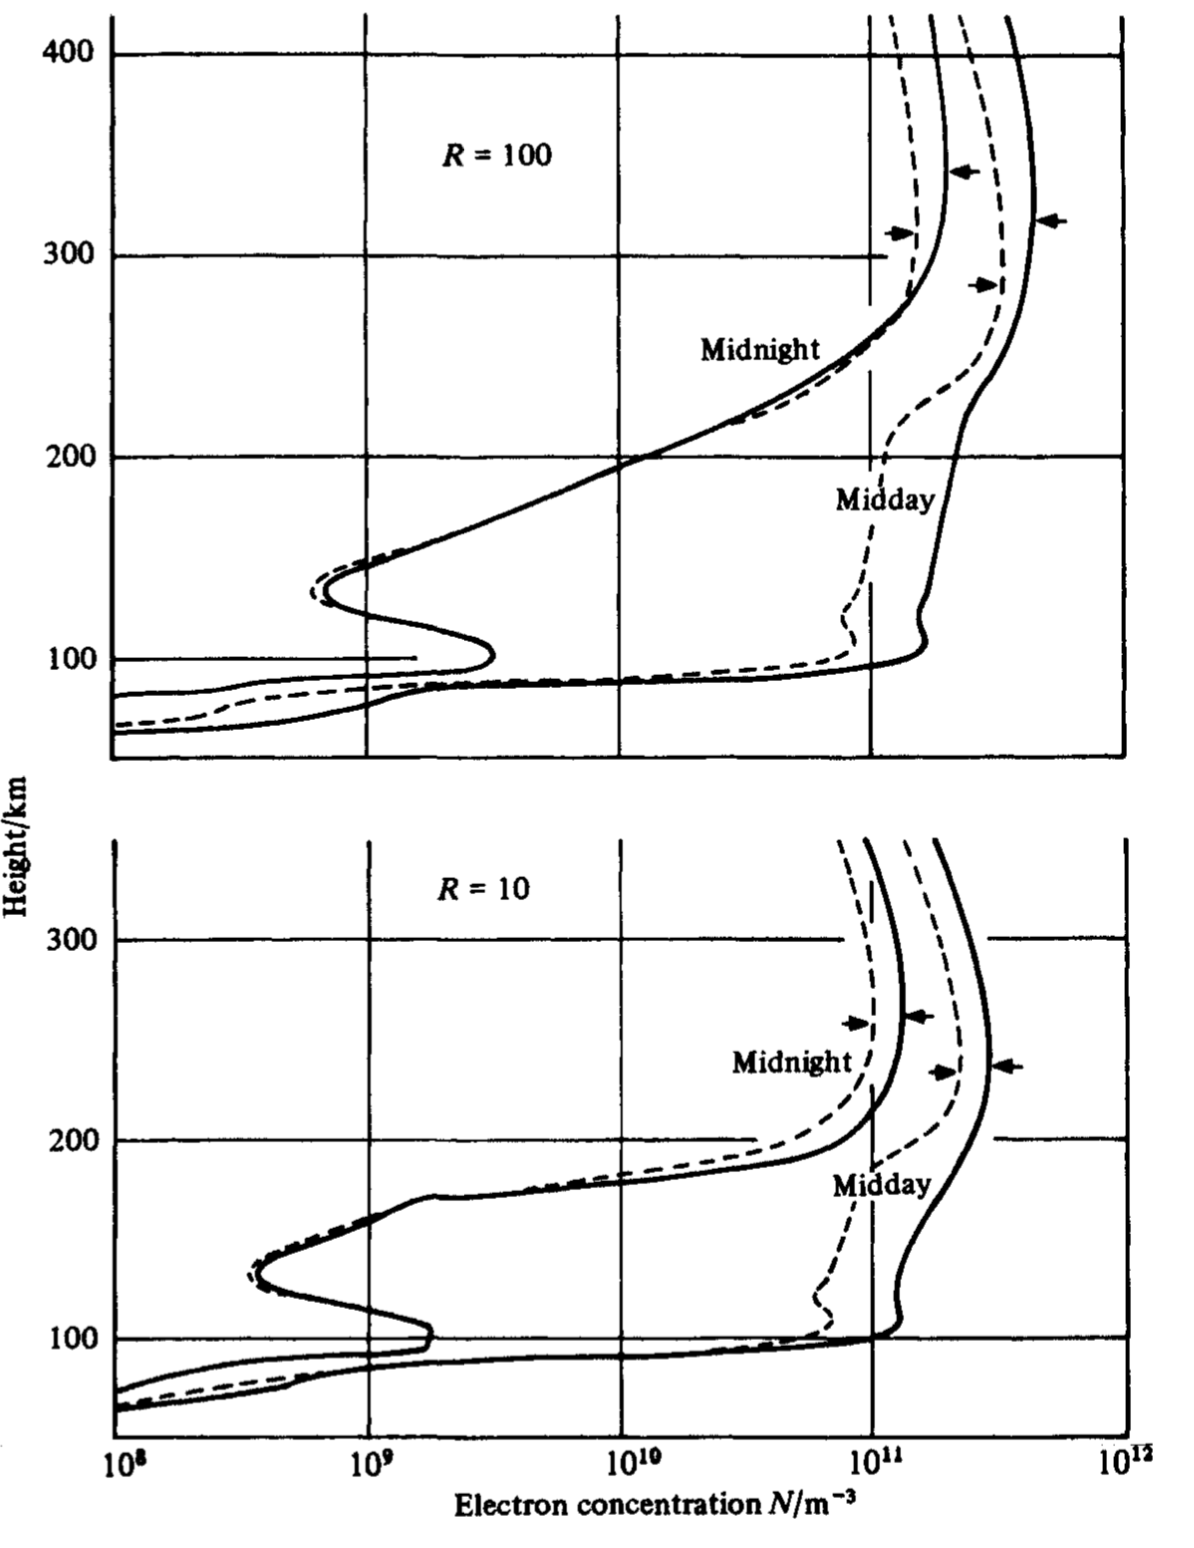
\includegraphics[width = 3in]{figs/structure_iono.png}
         \caption{}
    \label{fig:struct_ion} 
 \end{subfigure}
\qquad
 \begin{subfigure}[b]{0.44\textwidth}
         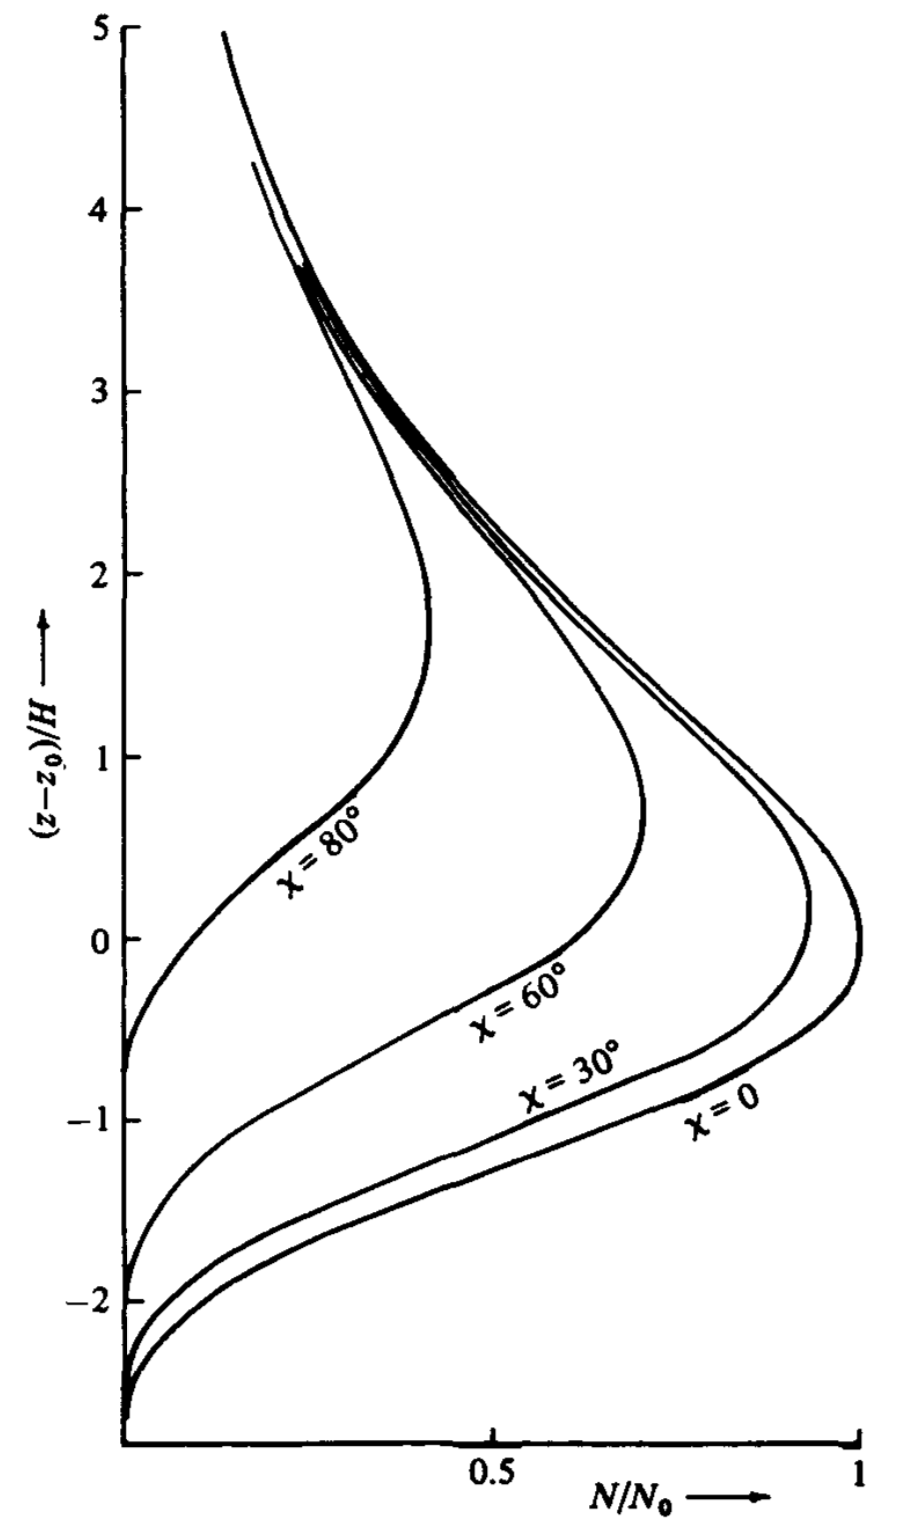
\includegraphics[width = 2.35in]{figs/chapman.png}
          \caption{ }
     \label{fig:chapman}
 \end{subfigure}
 \end{center}
 \caption{\textbf{(a)} The charge density as a function of height in the ionosphere. It also shows how the ionosphere changes at midnight and noon. Dashed lines are for January while solid lines are for June. Also given is the number of sunspots, $R$, at the time of data collection.  Figure is taken from K.G. Budden (1961).\cite{budden1988propagation} \textbf{(b)} Contour plot of the Chapman Law for various azimuthal angles of the incident sun. Figure taken from K.G. Budden (1988).\cite{budden1988propagation} }
 \label{fig:elect_density}
\end{figure}

As stated above, at a first approximation, we expect that the electron density, $N$, is only a function of the eight above the earth's surface height, $z$. More compactly, $N = N(z)$. 

    \subsubsection{Electron Density, $N(z)$} % (fold)
    \label{ssub:electron_density}
    Before we can calculate how radio-waves are reflected off of the ionosphere, we must model the ionosphere's electron density. In the early 1930's, a simple model for the electron density as a function was produced called the Chapman Law.\cite{chapman1931b,chapman1931a} 

    If we assume the Earth is constant in composition and temperature (as well as neglect the curvature of the earth\footnote{See \texttt{https://www.tfes.org/} for more information.}), then the density of the atmosphere, $\rho = \rho(z)$, is given by 
    \begin{equation}
        \rho(z) = \rho_0 e^{-M g z/ RT} = \rho_0 e^{- z/\kappa} 
        \label{eq:atm_den}
    \end{equation} where $ \kappa \equiv RT/Mg$, $\rho_0 \equiv \rho(0)$, $M$ is the average molecular weight, $g$ is the gravitational acceleration (assumed constant), $R$ is the universal gas constant,\footnote{Since all of us are ``physicists,'' we feel the need to note the definition of $R$: $R\equiv k_B N_A$ where $k_B$ is Boltzmann's constant and $N_A$ is Avogadro's number.} and $T$ is the temperature. The result of (\ref{eq:atm_den}) comes by balancing the forces acting on infinitesimal layers of atmosphere that, on a whole, is taken to be static and solving the barometric equation.\cite{schroeder1999introduction}
    
    Next, we must find the intensity of the sun that passes through the earth's atmosphere. The intensity of the sun---not surprisingly---decreases as it goes through the atmosphere.\cite{budden1961radio} Since, the sun enters at an angle from the zenith, $\alpha$. By drawing a simple diagram,\footnote{Remember, we have a flat Earth; this is a subtle but important point in this derivation.} we can see that the area normal to the incident radiation of the sun will be a factor of secant too large than the area that the ground actually receives, i.e. $dA = dA_\perp \cos\alpha.$ Since intensity is inversely proportional to $dA$, we will have the relationship of 
    \begin{equation}
        dI = I \sigma \rho \sec(\alpha) \, dz.
        \label{eq:diff_intensity}
    \end{equation}
    where $\sigma$ is a mass coefficient of absorption of the atmosphere. If we plug (\ref{eq:atm_den}) into (\ref{eq:diff_intensity}) and integrate, we get
    \begin{align}
        I(z)&= I_0 \exp\left[ -\sigma \kappa  \rho_0 \sec(\alpha) e^{- z/\kappa}\right] = I_0 \exp\left[ - \sec(\alpha) e^{- (z - z_0)/\kappa}\right]
        \label{eq:inten_v_height}
    \end{align}
    if we (cleverly) define $z_0 \equiv \kappa \ln \left(\sigma \kappa  \rho_0\right)$. The rate of absorption of energy at height $z$ is $\cos(\alpha)(dI/dz)$. If we assume that the rate of production of electrons, $q$, is proportional to this, then we get 
    \begin{equation}
        q(z) = q_0 \exp\left[1 - \frac{z-z_0}{\kappa} - \sec(\alpha) e^{- (z - z_0)/\kappa}\right].
        \label{eq:rate_prod_elec}
    \end{equation}

    Empirically---at least in the D and E-layers of the ionosphere\footnote{In the F-layer, this rate law may be equal to $dN/dt = q - b N$, but for the sake of simplicity we do not treat it as such.}---the variation of charge density is given by\cite{budden1961radio}
    \begin{equation}
        \frac{dN}{dt} = q - a N^2
        \label{eq:charge_den_rate}
    \end{equation}
    where $a$ is a ``recombination constant.'' In the steady-state solution, where $dN/dt \approx 0$, we have $N = \sqrt{q/a}$ or
    \begin{equation}
        N(z) = N_0 \exp\left[\frac12\left(1 - \frac{z-z_0}{\kappa} - \sec(\alpha) e^{- (z - z_0)/\kappa}\right)\right]
        \label{eq:chapman}
    \end{equation}
    where $N_0$ is a constant we can gather from experimental data. Quite simply, (\ref{eq:chapman}) is the Chapman Law.\cite{chapman1931a,chapman1931b,budden1961radio,budden1988propagation}


    % subsubsection electron_density (end)
    
    \subsubsection{A Modified Chapman Law, $\overline N(z,t)$} % (fold)
    \label{ssub:modified_chapman_law}
    Unfortunately, the Chapman Law is a rather simple model. It is not time dependent. It is also almost entirely qualitative due to the $\sigma$ constant that is highly dependent on what chemical species are in the atmosphere and the energy of incident light. However, it provides a good starting place to begin modifying for more accurate and simulations.

    Clearly, Fig.\ref{fig:struct_ion} demonstrates that the electron density of the ionosphere changes as a function season and time of day. In order to make the Chapman Law model of the time dependent, we can add a time dependent factor out front. To put another way, $\overline N(z,t) = T(t) N(z)$. A simple approximation is to make $T(t)$ linearly dependent on time. If we let
    \begin{equation}
        T(t) = 1 + d(t) + s(t)
        \label{eq:time_dep}
    \end{equation}
    where $d(t)$ is the ionosphere dependence on the time of day and $s(t)$ is the dependence on the season. From Fig.\ref{fig:struct_ion} we restrict the range of $d(t)$ and $s(t)$, where $d(t) \in [0,1]$ and $s(t) \in [0,4]$, respectively. These range restrictions were chosen as Fig.\ref{fig:struct_ion} demonstrates that seasonal dependence is more important than the time of day by roughly a factor of four. In our model, we input a sawtooth function for both $s(t)$ and $d(t)$ with each function's respective range. At midday, $s(t_{noon}) = 1$ and at midnight $s(t_{mid}) = 0$. Similarly, $d(t_{dec}) = 4$ while $d(t_{jun}) = 0$.\footnote{Since we are focusing our attention near South America, the most intense solar radiation comes in the summer months, which is December for our friends in the Southern Hemisphere.}

    In all, the electron-density as a function of height and time where $\overline N(t,z)$ is given by 
    \begin{align}
        \overline N(z,t) &= T(t)N(z) \nonumber \\
        &= N_0(1 + d(t) + s(t))\exp\left[\frac12\left(1 - \frac{z-z_0}{\kappa} - \sec(\alpha) e^{- (z - z_0)/\kappa}\right)\right]
        \label{eq:final_eden}
    \end{align}
    which is a simple, analytic model for the ionosphere that is used in our model.
    % subsubsection our_modified_chapman_law (end)

    \subsubsection{The Index of Refraction of the Ionosphere} % (fold)
    \label{ssub:index_of_refraction}

    To understand how to radio-waves will interact with the ionosphere, we must find an expression for the refractive index of light through the plasma. For simplicity, we are going to consider the ionosphere to be made of electrons that do not collide with one another and is isotropic throughout. When we do this, we can derive a relatively simple expression for the index of refraction of light through the medium.

    Simply put, the index of refraction relates how fast an electromagnetic wave is able to pass through a medium.\cite{jackson1999classical,townsend2000modern} We denote the index of refraction of a medium with the letter $n$; if $n = 1$ then the ray of light is moving at one of Nature's fundamental constants, $c.$

    To derive an expression for $n$ in an isotropic medium without electron collisions, we look at Maxwell's equations. In any upper-level textbook on Classical Electrodynamics, we have (from Faraday's Law of Induction)
    \begin{subequations}
           \begin{align}
       & \nabla \times \mathbf{E} = -i k \mathcal{H} \\& \nabla \times \mathcal{H} = \frac{ik}{\epsilon_0} \mathbf{D} 
    \end{align} 
    \label{eq:curls}
    \end{subequations}

    where $k$ is the wavenumber defined as $k = 2\pi/\lambda$ (where $\lambda $ is the wavelength of light), $\mathcal{H} = Z_0 \mathbf{B}$ (where $Z_0 \equiv \mu_0/\epsilon_0$ is the characteristic impedance of free space and $\mathbf{B}$ is the external magnetic field\footnote{In this case, the Earth's. Near South America, this value is $|\mathbf{B}| \approx 47 \si{\micro\tesla}$.\cite{maus2010us}}), and $\mu_0$ and $\epsilon_0$ are the permeability and permitivity of free space, respectively.\cite{jackson1999classical,griffiths2005introduction}
    % subsubsection index_of_refraction (end)

    If we are describing a progressive plane wave,\footnote{This simply means that there is no $x$ or $y$-dependence when the waves are traveling in the $z$-direction (for Cartesian coordinates). Since we haven't chosen any coordinate system, we are free to choose any direction that $z$ points in.} we have
    \begin{align}
         \frac{\partial}{\partial x} = \frac{\partial}{\partial y} = 0, \qquad \frac{\partial}{\partial z} = -i k n
        \label{eq:plane_wave}
    \end{align}
    which when combined with equations (\ref{eq:curls}) we find
    \begin{subequations}
     \begin{align}
        \mathcal{H}_x &= - n E_y \\
        \mathcal{H}_y & = nE_x \\
        \mathcal{H}_z & = 0
    \end{align}
    \label{eq:int_step}
    \end{subequations}
    Neglecting any damping, Newton's second law can relate the electric polarization, $\mathbf{P} = Ne\mathbf{r}$ and electric field via
    \begin{align}
         &\frac{Ne}{m}\mathbf{E}e = \frac{\partial^2 \mathbf{P}}{\partial t^2}
         &\Rightarrow \mathbf{P} = -\frac{Ne^2}{m\omega^2}\mathbf{E}
         \label{eq:elec_polar}
     \end{align} 
     where we utilized the fact that the electric field varies with a phase factor, implying that $\partial^2/\partial t^2 = -\omega^2$.\cite{budden1961radio,budden1988propagation} 

     Using (\ref{eq:elec_polar}), defining $X \equiv  N e^2/\epsilon_0m \omega^2$, and enforcing our plane-wave relations of (\ref{eq:plane_wave}) we get 
     \begin{subequations}
         \begin{align}
             n \mathcal{H}_y &= E_x(1 - X) \\
            -n \mathcal{H}_x &= E_y(1 - X) \\
            0 &= E_z
         \end{align}
     \end{subequations}
     which, when utilizing equations (\ref{eq:int_step}), we can find the refractive index as
     \begin{equation}
          n^2 = 1 - X = 1 - \frac{N e^2}{\epsilon_0 m \omega^2}
      \end{equation}
      which is independent in of the direction that the radio-wave travels, but is dependent on its frequency and some fundamental constants.\footnote{So long as the radio-wave is purely a transverse wave and has no longitudinal component or the longitudinal component is negligible, this holds.}

% subsection the_ionosphere (end)

\subsection{The Ocean} % (fold)
\label{sub:the_ocean}

\subsubsection{Data Collection} % (fold)  
\label{ssub:data_collection}

\subsubsection{Curve Fitting} % (fold)
\label{ssub:curve_fitting}

% subsubsection curve_fitting (end)

% subsubsection data_collection (end)
% subsection the_ocean (end)

% section model (end)

\section{Results} % (fold)
\label{sec:results}

 \subsection{Problem I: A Turbulent Ocean} % (fold)
 \label{sub:part_i}

 \subsection{Problem II: The Japanese Alps} % (fold)
 \label{sub:part_ii}
 
 \subsection{Problem III: A Message to a Boat} % (fold)
 \label{sub:part_iii}
 
 % subsection part_iii (end)
 % subsection part_ii (end)
 
 % subsection part_i (end)
% section results (end)

\section{Conclusion}
\label{sec: conclusion}

\section*{Acknowledgments}
\label{sec: acknowledge}


%%%%%%%%%%%%%%%%%%%%%%%%%%%%%%%%%%%%%%%%%%%%%%%%%%%%%%%%%%%%%%%%%%%%%%%
%% Bibliography
%%%%%%%%%%%%%%%%%%%%%%%%%%%%%%%%%%%%%%%%%%%%%%%%%%%%%%%%%%%%%%%%%%%%%%%
\newpage 

% \nocite{*}
\bibliographystyle{plainnat}
\bibliography{solution}

\end{document}
